\chapter{Competencias y Estrategia de Mercado}\label{chapter05}

Se aplican herramientas de análisis estratégico para posicionar el proyecto frente a la competencia. Este capítulo es complementario al núcleo técnico-investigativo del PFI (arquitectura y score de tendencia en el Capítulo 1, requerimientos en el Capítulo 3, User Research en el Capítulo 6 y validación empírica en el Capítulo 7): aporta contexto de mercado, pero no reemplaza ni condiciona las decisiones técnicas del sistema.

\section{Análisis FODA}

\begin{table}[ht]
	\centering
	\caption{Análisis FODA -- Fortalezas y Debilidades}
	\label{tab:foda-fd}
	\begin{tabularx}{\textwidth}{@{}X X@{}}
		\toprule
		\textbf{Fortalezas} & \textbf{Debilidades} \\
		\midrule
		Uso de API oficial (datos confiables y legales). Score de tendencia propio basado en histórico. &
		Dependencia de límites de la API oficial. Sin datos de otras plataformas (solo Mercado Libre). \\
		\bottomrule
	\end{tabularx}
\end{table}

\begin{table}[ht]
	\centering
	\caption{Análisis FODA -- Oportunidades y Amenazas}
	\label{tab:foda-oa}
	\begin{tabularx}{\textwidth}{@{}X X@{}}
		\toprule
		\textbf{Oportunidades} & \textbf{Amenazas} \\
		\midrule
		Creciente uso de marketplaces en Argentina. Vendedores sin herramientas de anticipación de demanda. &
		Cambios en política de acceso a la API de Mercado Libre. Aparición de herramientas similares por parte de la propia plataforma. \\
		\bottomrule
	\end{tabularx}
\end{table}

\section{Cruz de Porter (5 fuerzas)}

\begin{itemize}
	\item \textbf{Rivalidad entre competidores}: media -- existen soluciones genéricas (Google Trends) pero ninguna enfocada en Mercado Libre Argentina.
	\item \textbf{Poder de negociación de clientes}: alto -- vendedores pueden optar por no usar ninguna herramienta y decidir de forma manual.
	\item \textbf{Poder de negociación de proveedores}: alto -- el proyecto depende completamente de la API oficial de Mercado Libre.
	\item \textbf{Amenaza de nuevos entrantes}: media -- la barrera técnica es moderada, pero la especialización en el marketplace local es un diferencial.
	\item \textbf{Amenaza de productos sustitutos}: media -- hojas de cálculo manuales o seguimiento intuitivo por parte de vendedores.
\end{itemize}

\begin{figure}[H]
	\centering
	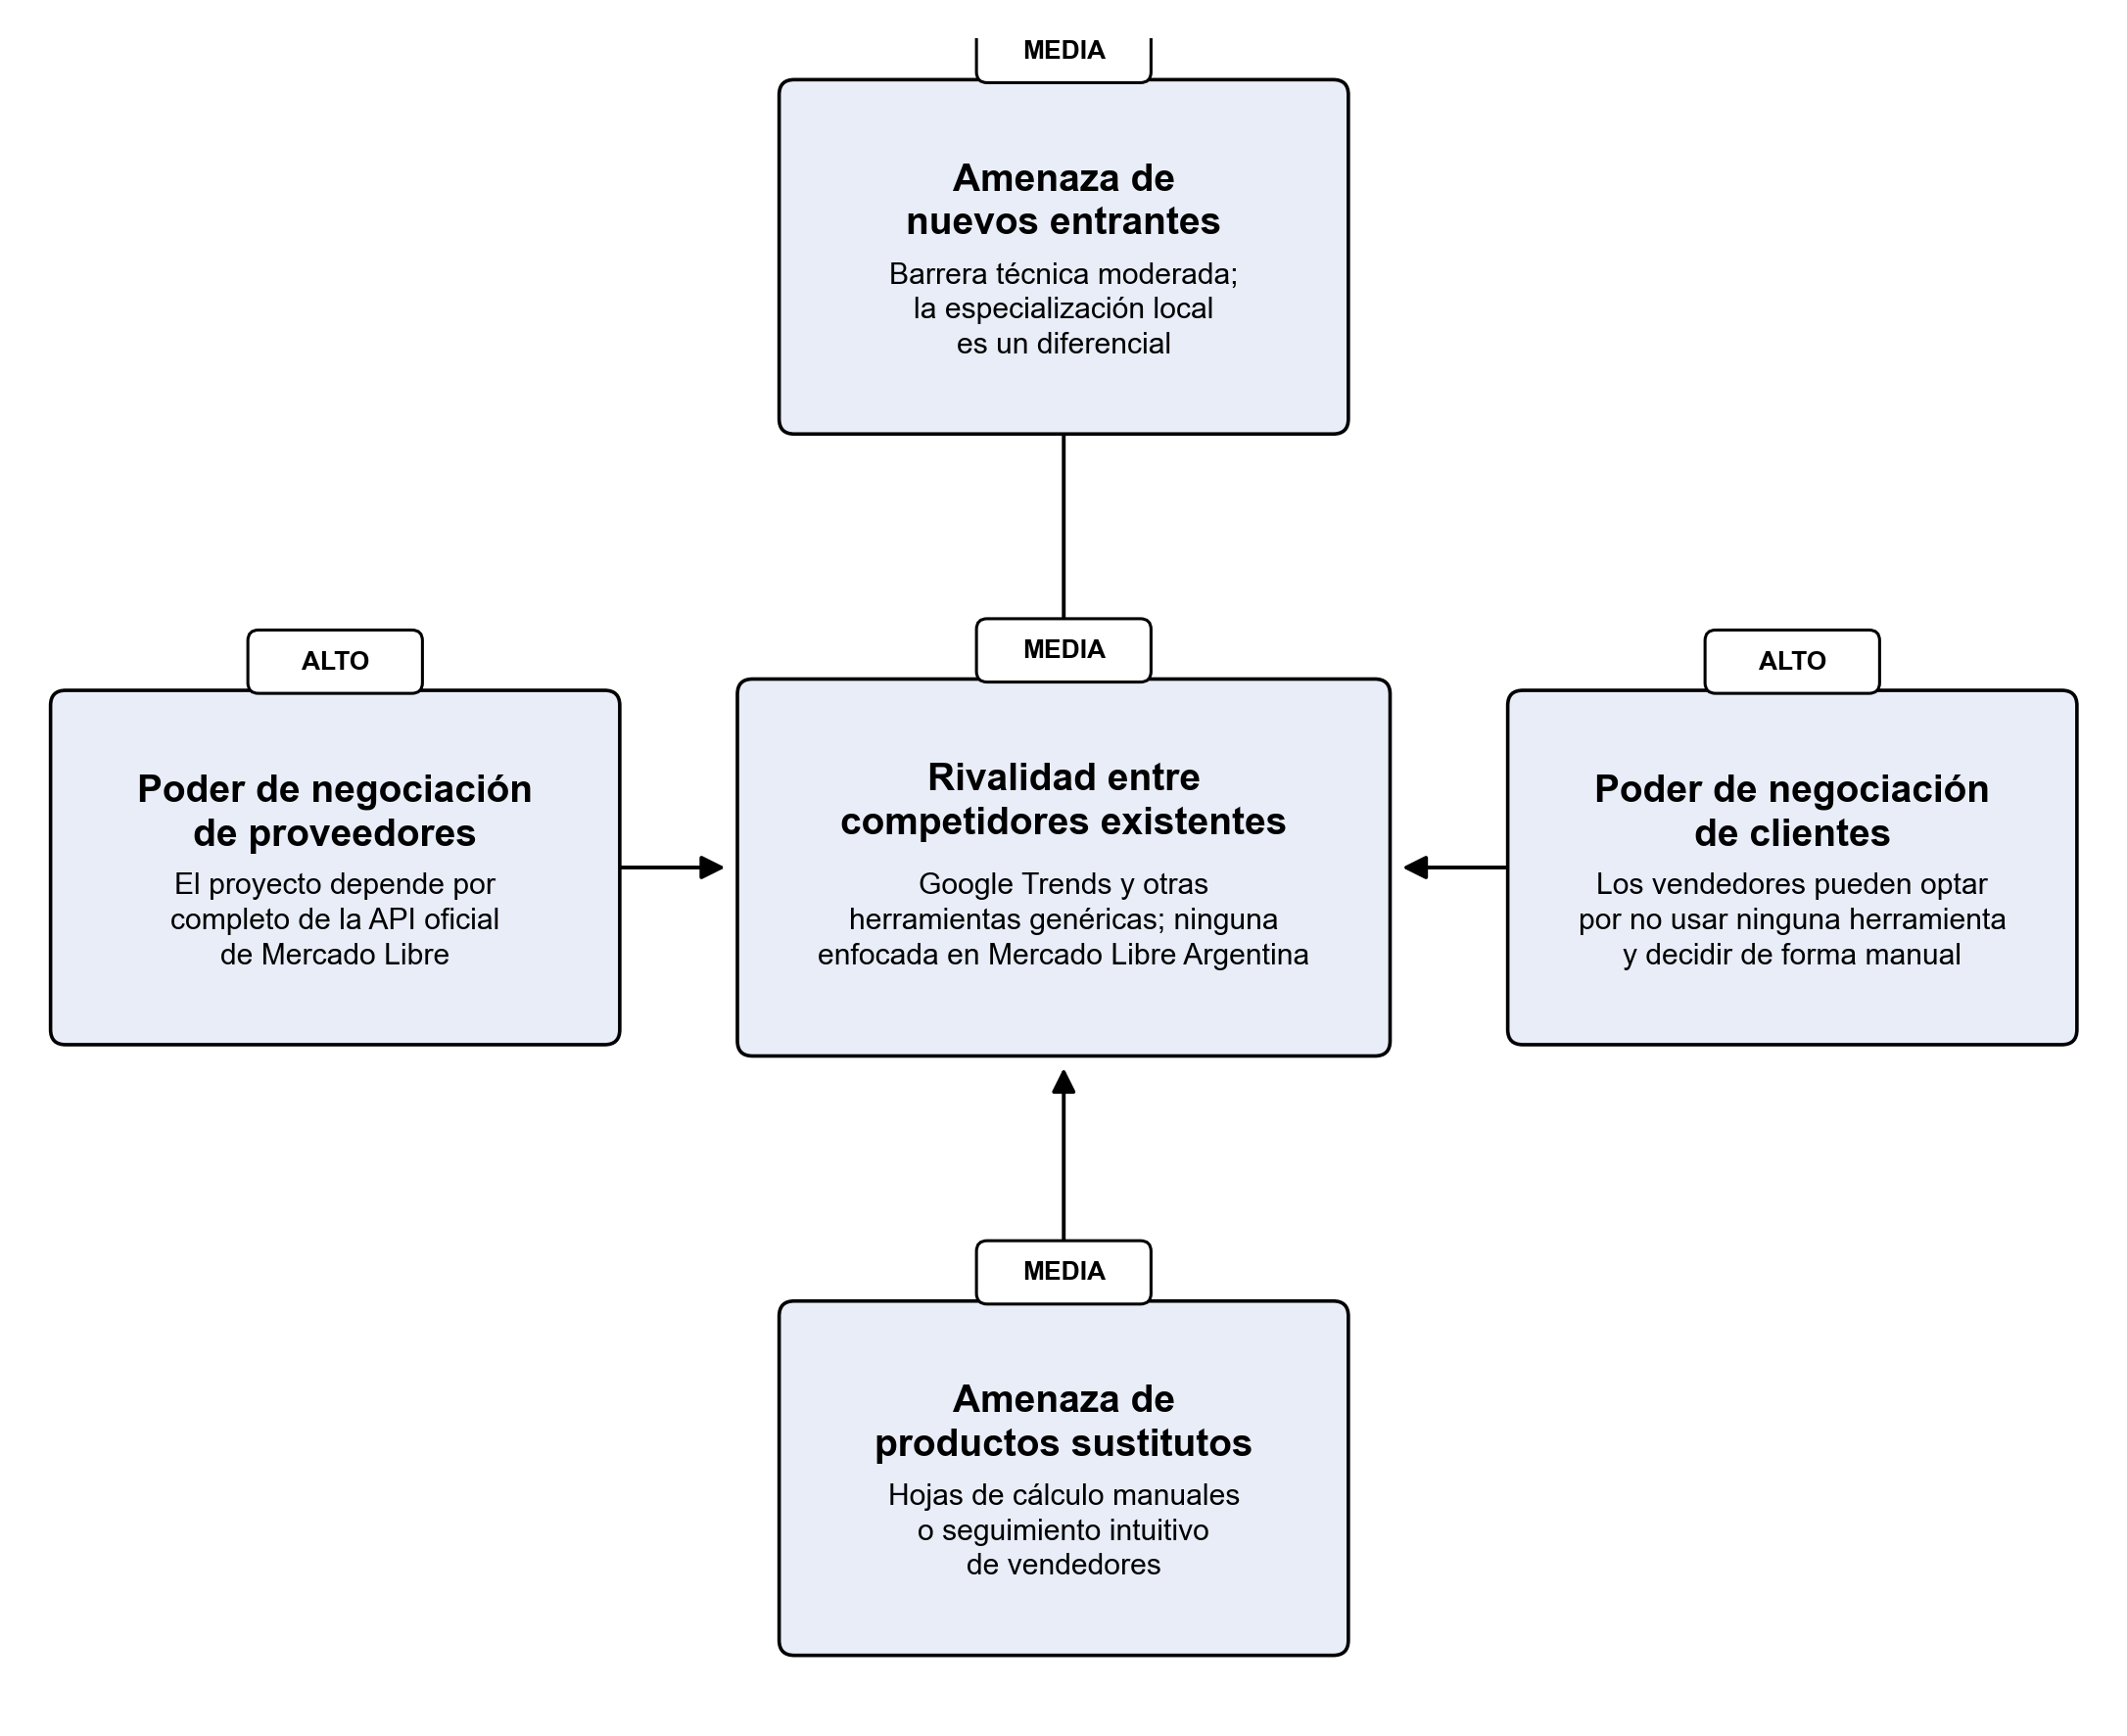
\includegraphics[width=0.95\textwidth]{./images/diagramas/diagrama_porter.png}
	\caption{Cruz de Porter (5 fuerzas) aplicada al proyecto.}
	\label{fig:diagrama-porter}
\end{figure}

\section{Triple P (Producto, Precio, Plaza)}

\begin{itemize}
	\item \textbf{Producto}: plataforma de detección temprana de productos en tendencia dentro de Mercado Libre, con dashboard y alertas.
	\item \textbf{Precio}: modelo freemium -- funciones básicas gratuitas y alertas/segmentación avanzada bajo suscripción mensual (desarrollado en la Sección~\ref{sec:modelo-negocio}).
	\item \textbf{Plaza}: acceso vía web, dirigido a vendedores PyME y particulares que operan en Mercado Libre Argentina.
\end{itemize}

\section{Modelo de negocio}\label{sec:modelo-negocio}

El modelo de negocio se apoya en el mismo segmento validado por el User Research (Capítulo~\ref{chapter06}): vendedores de Mercado Libre que hoy deciden qué stockear de forma intuitiva y manifestaron, en la encuesta, una disposición alta a adoptar una herramienta automatizada (68,9\,\% respondió ``Sí'' y 26,7\,\% ``Tal vez'').

\textbf{Propuesta de valor}: reducir el costo de detectar tarde una tendencia -- cuantificado por el vendedor entrevistado en una relación de rentabilidad de 3 a 1 respecto de haber tenido la señal dos semanas antes (Entrevista 1, Anexo D) -- mediante alertas y un score de tendencia auditable, en lugar de un ranking genérico sin desglose.

\textbf{Segmentos}: (a) vendedores individuales y PyME de Mercado Libre Argentina, segmento primario validado por la encuesta y las tres entrevistas; (b) agencias o gestores que administran varias cuentas de venta, como segmento secundario a explorar en una etapa posterior, sin validación propia todavía.

\textbf{Flujos de ingreso}: modelo freemium por suscripción mensual. El nivel gratuito ofrece el ranking y el dashboard con alcance acotado; el nivel pago -- validado en la Entrevista 2 en un rango de USD 10 a 30 mensuales (Anexo D) -- desbloquea alertas en tiempo real, historial completo y exportación sin límites.

\textbf{Canales}: adquisición orgánica a través de las mismas comunidades que ya usan los vendedores para intercambiar información. El grupo de WhatsApp de vendedores mencionado en la Entrevista 1 es, en los propios términos del entrevistado, el canal que más le aportó de todos los que probó, por encima de planillas propias o de seguir cuentas -- una señal directa de por dónde captar los primeros usuarios.

\textbf{Estructura de costos}: infraestructura cloud gestionada (Render y Supabase, Sección~\ref{sec:evidencia-cuantitativa}), comisión de la pasarela de pago sobre los ingresos, y un presupuesto de soporte y marketing continuo. No se contempla costo de personal más allá del equipo fundador actual.

\textbf{Sustentabilidad}: al ser un producto de software con costo marginal casi nulo por usuario adicional -- la infraestructura actual ya sostiene 162 productos y 3911 scores calculados sin necesidad de escalar (Sección~\ref{sec:evidencia-cuantitativa}) --, el margen de contribución por suscriptor es alto una vez cubiertos los costos fijos. El punto de equilibrio y los escenarios de rentabilidad se desarrollan en la Sección~\ref{sec:viabilidad-economica}.

\section{Viabilidad económico-financiera}\label{sec:viabilidad-economica}

Se evalúa la viabilidad económica del modelo de negocio mediante punto de equilibrio, Valor Actual Neto (VAN), Tasa Interna de Retorno (TIR) y período de recupero (\emph{payback}), sobre un horizonte de 24 meses y bajo los siguientes supuestos declarados:

\begin{itemize}
	\item \textbf{Precio de suscripción}: USD 15 mensuales, dentro del rango de USD 10 a 30 que el vendedor entrevistado consideró razonable (Entrevista 2, pregunta 9, Anexo D), elegido en el extremo conservador del rango.
	\item \textbf{Costos fijos mensuales}: USD 32 de infraestructura (Render y Supabase, según tarifas publicadas al momento de este informe -- a reverificar antes de la entrega final) más USD 60 de soporte y marketing continuo.
	\item \textbf{Costo variable}: comisión de pasarela de pago del 6\,\% sobre los ingresos por suscripción.
	\item \textbf{Inversión inicial}: USD 2000, que cubren identidad de marca, lanzamiento en las comunidades de vendedores identificadas como canal (Sección~\ref{sec:modelo-negocio}) y un colchón operativo de los primeros meses.
	\item \textbf{Tasa de descuento}: 1,5\,\% mensual (aprox. 18\,\% anual), consistente con el riesgo de un proyecto en etapa temprana en un mercado emergente.
	\item \textbf{Adopción}: dos escenarios de cantidad de suscriptores pagos, con una rampa lineal durante los primeros 6 meses y una meseta estable después. No se proyecta a partir del tamaño total del universo de vendedores de Mercado Libre Argentina, ya que no se dispone de una fuente pública confiable de esa cifra al momento de este informe -- los escenarios se construyen como cotas razonables (piso y techo) y no como una estimación de participación de mercado.
\end{itemize}

\begin{table}[H]
	\centering
	\caption{Escenarios de viabilidad económica}
	\label{tab:viabilidad-economica}
	\begin{tabularx}{\textwidth}{@{}>{\raggedright\arraybackslash}p{4.4cm} X X@{}}
		\toprule
		\textbf{Indicador} & \textbf{Pesimista} (meseta: 40 suscriptores) & \textbf{Optimista} (meseta: 150 suscriptores) \\
		\midrule
		Punto de equilibrio & \multicolumn{2}{p{7.6cm}}{7 suscriptores pagos por mes (cubre los USD 92 de costos fijos mensuales)} \\
		Flujo neto mensual en meseta & USD 472 & USD 2023 \\
		Período de recupero (\emph{payback}) & Mes 8 & Mes 4 \\
		VAN a 24 meses (tasa 1,5\,\% mensual) & USD 6092 & USD 33414 \\
		TIR mensual & 15,0\,\% & 45,7\,\% \\
		\bottomrule
	\end{tabularx}
\end{table}

Ambos escenarios muestran VAN positivo y recupero de la inversión inicial dentro del primer año, lo que respalda la viabilidad económica del modelo bajo los supuestos declarados. La TIR mensual es alta porque se trata de un producto de software con costo marginal casi nulo por usuario adicional y una inversión inicial acotada; por ese mismo motivo, anualizarla por interés compuesto produce un número con escaso valor interpretativo (una inversión inicial pequeña frente a un flujo de caja mensual sostenido infla artificialmente la tasa), por lo que se prioriza el VAN y el \emph{payback} como indicadores de decisión, en lugar de reportar esa TIR anualizada.

Como limitación del análisis, el modelo no proyecta el tamaño total del mercado direccionable -- no existe, al momento de este informe, una fuente pública confiable sobre el número de vendedores activos de Mercado Libre en Argentina -- ni incluye costo de personal más allá del equipo fundador actual. Ambos supuestos deberán revisarse si el proyecto avanza hacia una operación comercial real.

\section{Branding y logotipo}

\textbf{Nombre}: el producto se identifica comercialmente como \textbf{Tendar} -- de ``tendencia'' + ``radar'' --, elegido deliberadamente sin ninguna referencia a Mercado Libre en el nombre. Esta decisión responde a una observación de la instancia de revisión oral del hito del 50\,\%: atar la marca al nombre de la plataforma sobre la que opera hoy dejaría al producto sin identidad propia ante un cambio en las condiciones de acceso a esa API, riesgo ya identificado en el análisis FODA (Tabla~\ref{tab:foda-oa}) y en la Cruz de Porter (Figura~\ref{fig:diagrama-porter}). El título académico del proyecto (portada) se mantiene sin cambios, ya que corresponde a la Propuesta de Tema aprobada por la cátedra (Anexo A); Tendar es el nombre bajo el cual el producto se presentaría comercialmente.

\begin{figure}[H]
	\centering
	
\includegraphics[width=0.85\textwidth]{./images/diagramas/logo_tendar.png}
	\caption{Logotipo de Tendar.}
	\label{fig:logo-tendar}
\end{figure}

\textbf{Logotipo} (Figura~\ref{fig:logo-tendar}): el isotipo combina un radar -- círculos concéntricos con un sector de barrido -- con una línea de tendencia ascendente que se despega del punto detectado: una traducción visual directa de lo que hace el sistema, detectar una señal temprano (el radar) y mostrar que está despegando (la línea ascendente), en lugar de un ícono genérico de gráfico de barras o de carrito de compras. La paleta de azules es consistente con el resto de las figuras del documento (diagramas de arquitectura, Cruz de Porter), para mantener una identidad visual única entre el sistema y el informe que lo documenta.

\textbf{Tagline}: ``radar de tendencias'' -- resume la propuesta de valor (Sección~\ref{sec:modelo-negocio}) en tres palabras: detección (radar) del objeto central del negocio (tendencias).

\textbf{Tono de comunicación}: directo y cuantitativo, sin adjetivos vacíos, consistente con el hallazgo de la Entrevista 2 de que el score necesita explicabilidad para generar confianza (Sección~\ref{sec:pruebas}). La comunicación de marca evita promesas genéricas del tipo ``sabé lo que se viene'' y en cambio se apoya en números concretos -- el score, su desglose, el ejemplo real de la Sección~\ref{sec:score-formal} --, replicando en la comunicación la misma lógica de transparencia que ya tiene el producto.
